%%
%% Berliner Hochschule für Technik --  Projektarbeit/Projekt-Labor
%%
%% Chapter 1
%%
%%


\chapter{Introduction}

The scope of the project is to produce a algorithm, which outputs the current state of charge (SoC) of the lead acid batterie attached to the charge controller (MPPT-HUS1510). 

The git source code repository of this document  \cite{Schons_Development_and_validation_2021} is available at \footnote{ \url{https://github.com/mulles/Doc_Projekt-Labor_SOC} }

\section{Background}

\cite{espedal2021current}  Current Trends for State-of-Charge (SoC) Estimation in

Lithium-Ion Battery Electric Vehicles.

The kalman filter is a great tool to base a SoC algorithms on, as it is clearly defined by mathematical theories more than by a arbitrary algorithm designed by a programmer. One needs to use a extend kalman filter as the problem to solve is non linear, TODO explain why it is non linear. 

Other methods are based on auto regressive exogenous (ARX) model or a combination of it and the Kalman Filter. TODO reference to resources.

There are 3 main approaches: model-based, data-driven, coulomb-counting. 

\subsubsection{Current integration method - Coulomb Counting}

Seems the most simple way to define SoC:

\begin{equation}
z( {z(0)},{{i}}(t),\Delta{t}) = z(0) - \frac{1}{{Q_{C}}}\int_{0}^{\Delta t} {i(t)\ dt}
\end{equation}
where: 
\begin{tabbing}
\phantom{$v(t)  \  \ \ \ $}\= \kill
$z  $\> = the SoC  \\
$i  $\> = battery current  \\
$Q_{C}$\> =  battery capacity   \\
\end{tabbing}

The initial SoC $z(0)$ is determined by OCV lookup table. Starting from there the charge in relation to total capacity entering and leaving the battery is subtracted from SoC. This method has several disadvantages: \\

-The initial SoC incorpated already an error, which won't be corrected in the process \\
-Error in counting and measurement errors accumalte quite quickly\\
-The algorithms only recalibrate on full charge, which especially in solar systems does not occur regularly, producing awful SoC till recalibration. \\

The coulomb counting method it most often combined with voltage measurements, while battery is at rest and a resulting OCV-lookup. This mitigates the recalibration problem in case the battery gets some rests. Furthermore hysteresis is not taken into account with this enhancement. TODO cite Gregory. %But as OCV-SoC curve is very flat for mid range SoC it does not help to much overall.


\begin{pylabcode}[plotsession]
rc('text', usetex=True)
rc('font', **{'family':'serif', 'serif':['Times']})
rc('font', size=10.0)			
rc('legend', fontsize=10.0)
xData = [ 0, 1000, 2000, 3000, 4000, 5000, 6000, 7000, 8000, 9000, 10000, 11000, 12000, 13000, 14000, 15000, 16000, 17000, 18000, 19000, 20000, 21000, 22000, 23000, 24000, 25000, 26000, 27000, 28000, 29000, 30000, 31000, 32000, 33000, 34000, 35000, 36000, 37000, 38000, 39000, 40000, 41000, 42000, 43000, 44000, 45000, 46000, 47000, 48000, 49000, 50000, 51000, 52000, 53000, 54000, 55000, 56000, 57000, 58000, 59000, 60000, 61000, 62000, 63000, 64000, 65000, 66000, 67000, 68000, 69000, 70000, 71000, 72000, 73000, 74000, 75000, 76000, 77000, 78000, 79000, 80000, 81000, 82000, 83000, 84000, 85000, 86000, 87000, 88000, 89000, 90000, 91000, 92000, 93000, 94000, 95000, 96000, 97000, 98000, 99000, 100000 ]
yData = [ 11640, 11653, 11666, 11679, 11692, 11706, 11719, 11732, 11745, 11758, 11772, 11785, 11798, 11811, 11824, 11838, 11851, 11864, 11877, 11890, 11904, 11917, 11930, 11943, 11956, 11970, 11983, 11996, 12009, 12022, 12036, 12049, 12062, 12075, 12088, 12102, 12115, 12128, 12141, 12154, 12168, 12181, 12194, 12207, 12220, 12234, 12247, 12260, 12273, 12286, 12300, 12313, 12326, 12339, 12352, 12366, 12379, 12392, 12405, 12418, 12432, 12445, 12458, 12471, 12484, 12498, 12511, 12524, 12537, 12550, 12564, 12577, 12590, 12603, 12616, 12630, 12643, 12656, 12669, 12682, 12696, 12709, 12722, 12735, 12748, 12762, 12775, 12788, 12801, 12814, 12828, 12841, 12854, 12867, 12880, 12894, 12907, 12920, 12933, 12946, 12960 ]
x = []
y = []
for OCV in xData:
    x.append(OCV / 1000)
for SoC in yData:
    y.append(SoC / 1000)
 
figure(figsize=(3.25,2))
plot(x,y)
xlabel(r'SoC(\%)')
ylabel(r'OCV(V)')
savefig('OCVlead.pdf', bbox_inches='tight')
\end{pylabcode}

\begin{figure}[!ht]
\centering
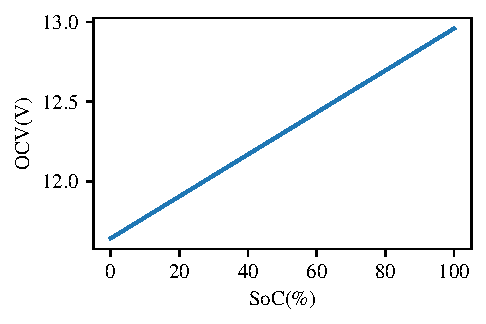
\includegraphics{OCVlead}
\caption{\label{fig:OCVLead} OCV Lead Acid }
\end{figure}



\begin{pylabcode}[plotsession]
rc('text', usetex=True)
rc('font', **{'family':'serif', 'serif':['Times']})
rc('font', size=10.0)			
rc('legend', fontsize=10.0)
xData = [ 0, 1000, 2000, 3000, 4000, 5000, 6000, 7000, 8000, 9000, 10000, 11000, 12000, 13000, 14000, 15000, 16000, 17000, 18000, 19000, 20000, 21000, 22000, 23000, 24000, 25000, 26000, 27000, 28000, 29000, 30000, 31000, 32000, 33000, 34000, 35000, 36000, 37000, 38000, 39000, 40000, 41000, 42000, 43000, 44000, 45000, 46000, 47000, 48000, 49000, 50000, 51000, 52000, 53000, 54000, 55000, 56000, 57000, 58000, 59000, 60000, 61000, 62000, 63000, 64000, 65000, 66000, 67000, 68000, 69000, 70000, 71000, 72000, 73000, 74000, 75000, 76000, 77000, 78000, 79000, 80000, 81000, 82000, 83000, 84000, 85000, 86000, 87000, 88000, 89000, 90000, 91000, 92000, 93000, 94000, 95000, 96000, 97000, 98000, 99000, 100000 ]
yData = [ 5000, 6266, 7434, 8085, 8531, 8867, 9134, 9355, 9543, 9705, 9847, 9974, 10088, 10191, 10285, 10372, 10451, 10525, 10595, 10659, 10720, 10777, 10831, 10882, 10931, 10977, 11021, 11063, 11104, 11142, 11180, 11216, 11251, 11284, 11317, 11349, 11379, 11409, 11438, 11467, 11495, 11522, 11548, 11574, 11600, 11625, 11650, 11675, 11699, 11723, 11746, 11769, 11793, 11815, 11838, 11861, 11883, 11906, 11928, 11950, 11972, 11994, 12017, 12039, 12061, 12083, 12105, 12127, 12150, 12172, 12195, 12217, 12240, 12263, 12286, 12309, 12333, 12356, 12380, 12404, 12428, 12452, 12477, 12501, 12526, 12552, 12577, 12603, 12629, 12655, 12682, 12708, 12735, 12763, 12790, 12818, 12846, 12875, 12903, 12931, 12960 ]
x = []
y = []
for OCV in xData:
    x.append(OCV / 1000)
for SoC in yData:
    y.append(SoC / 1000)
 
figure(figsize=(3.25,2))
plot(x,y)
xlabel(r'SoC(\%)')
ylabel(r'OCV(V)')
savefig('OCVLion.pdf', bbox_inches='tight')
\end{pylabcode}

\begin{figure}[!ht]
\centering
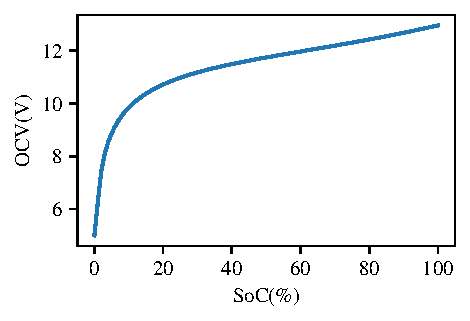
\includegraphics{OCVLion}
\caption{\label{fig:OCVLion} OCV Lithium }
\end{figure}

The current SoC function Charger::update\_soc \footnote{\url{https://github.com/LibreSolar/charge-controller-firmware/blob/5196694e42c38eee18ab25e65bd51ec578eba101/src/bat_charger.cpp\#L325}} of libre.solar only uses OCV-lookup function based on linear interpolation of 
ocv\_empty and  ocv\_full:

\begin{verbatim}
void Charger::update_soc(BatConf *bat_conf)
{
    static int soc_filtered = 0;       // SOC / 100 for better filtering

    if (fabs(port->current) < 0.2) {
        int soc_new = (int)((port->bus->voltage - bat_conf->ocv_empty) /
                   (bat_conf->ocv_full - bat_conf->ocv_empty) * 10000.0);

        if (soc_new > 500 && soc_filtered == 0) {
            // bypass filter during initialization
            soc_filtered = soc_new;
        }
        else {
            // filtering to adjust SOC very slowly
            soc_filtered += (soc_new - soc_filtered) / 100;
        }

        if (soc_filtered > 10000) {
            soc_filtered = 10000;
        }
        else if (soc_filtered < 0) {
            soc_filtered = 0;
        }
        soc = soc_filtered / 100;
    }

    discharged_Ah += -port->current / 3600.0F;   // charged current is positive: change sign
}
\end{verbatim}

\subsubsection{Equivalent circuit based models}
\
\
\
\begin{figure}[h!]
\begin{center}
\includegraphics{g10} %[trim=0.5cm 5.9cm 0.5cm 20cm]
\caption{\label{fig:ECMThevinModel} Equivalent circuit model }
\end{center} 
\end{figure} 
 \\
The figure \ref{fig:ECMThevinModel} is an empirical model known as Thévenin circuit-based battery model or equivalent circuit model (ECM), adhering to the equation: 

\begin{equation}
{v}(t) = {OCV}(z(t)) - {R}_{1} {i}_{R_1}(t) - {R}_{0} i(t)
\end{equation}
where: 
\begin{tabbing}
\phantom{$v(t)  \  \ \ \ $}\= \kill
$v$\> =  voltage measured on battery terminals under load   \\
$z  $\> = the SoC  \\
$OCV $\>  = a function based on a SoC-OCV lookup table \\
$R_1$\> = resistance due to \\
$C_1$\> = capacity due to \\
$R_0$\> = resistance due to \\
\end{tabbing}

The 



\subsubsection{Physics based models}

As Gregory Plettv puts it in his lectures notes of course ECE5720  \footnote{ \url{http://mocha-java.uccs.edu/ECE5720/ECE5720-Notes02.pdf}} :  "Battery management and controls using physics-based models is a major focus of our present research efforts and (I hope) of a future
course" in 2015. The first papers on the topic are available now \cite{9477587}, but Physics based models (PBM) still are hard to implement and not much material or software code is available. Thus the ECM model is preferred for now. Moreover, the PBM based models have a high computational complexity than
empirical models as ECM, making it non suitable for STMxxx. TODO find another citation of gregory plett


\subsubsection{Data-driven}

These approaches are based on artificial

intelligence (AI) and need good training data and the right training parameters. Combined with PBM's it is a very promising research field \cite{9477587}, which first successes to reduce the computational complexity so online estimation of SoC on MCU is	 possible.


\chapter{Implementation}

"A sigma-point Kalman filter is further used to manage inaccuracies generated by the reduction process and experimental-related issues such as measurement error (noise) in the current and voltage sensors."




Link to source code. \footnote{ \url{https://github.com/mulles/kalman-soc} } The algo is a fork of a kalman-soc from  Matthew Johnston of the company okra-solar. 

Some adjustments have been made to improve or adapt it to libre.solar use case and code base. 
 \\


Changelog: 



-adoption of libre solar code style guide 

-change of energy counting to coulomb counting

-use of float instead of integer in order to guarantee correct calculations, with no overflow. 

-

-exact changes are traceable with the commits to the fork. 
\\
\
\
\


{System's dynamic model} \\

The $f() $ function is defined as the $ f({\boldsymbol {x}}_{k},{\boldsymbol {i}}_{k},\Delta{t}) = {x}_{k} - \frac{1}{{Q_{C}}}\int_{0}^{\Delta t} {i_{k}\ dk} $ or more discrete $f({x}_{k},{i}_{k},\Delta{t}) = {x}_{k} - \frac{\Delta t}{Q_{C}} i_{k} $, thus current measurement $ {i}_{k} $ \\

The $h({\boldsymbol {x}}_{{k}})$ function is defined as the OCV lookup table. A general OCV lookup table for the battery chemistry can be used or for better results a specific OCV lookup table established by offline measurements for the given battery should be used. \\
To further improve the OCV prediction a correction of it can be performed by a equivalent circuit model (ECM) of the battery feed by the current measurement used to predict the SoC: 

\begin{equation}
{v}_{k} = {D} \ {OCV}({z}_{k}) + C {x}_{k}  +  D {i}_{k}  
\end{equation}
where:
\begin{tabbing}
\phantom{$v(t)  \  $}\= \kill
$C$\> =   $C= [0, -R_1, -R_2, ..., M] $ \\
$D$\> = $R_0 $    \\
\end{tabbing}


\section{Hardware Setup for validation}

\begin{figure}[!ht]
\includegraphics{SOC_Setup.png}
\caption{\label{fig:SoCSetup} Setup to verify SoC Algorithm}
\end{figure}



TODO Migrate from the other document.

TODO What resolution is necessary. 

\section{EKF Implementation}
date: (4d)

A good step by step guide to implement the extended kalman filter is \cite{rzepka2021implementing}.

To design an extended kalman filter algorithm three steps are necessary:
1.The control-input model and the observation model need to be well designed. 
2.The constants inside the models expressed as matrices need to be defined, which is as well known as parametrization of the model.  
3.The model needs to be implemented as code running on embedded systems. 

The key to success for a good SoC is a good definition of both models and a good parametrization. The implementation is independent of the use case and depends on the skills of the programmer, in his  hands lies the optimization of the  code. In case no FPU is available on the micro-controller unit (MCU) fix point arithmetic might be an option.  

Particularly challenging is the parametrization, which is typically done offline \footnote{not generated by the micro controller unit (MCU) the algorithm is deployed to, thus not on the system running the final algorithm. Offline means on more advanced hardware, which is not available in the final product. See \url{https://en.wikipedia.org/wiki/Online_model} } and requires quite advanced equipment. The Adaptive extend Kalman Filter (AEKF) is an option, where the parameters are determined online, but still AEKF needs to be initialized with parameters not necessary fitting all batteries of a given chemistry, because of different capacities or tolerances and specific designs. 
TODO It needs to be researched if it only affects the convergence time or if convergence is not reached at all? A further advantage of an adaptive filter is that the state of health (SOH) can be determined along the side. 
When simple observation and control-input models are used as in the okra kalman-soc algorithm, the parametrization might be much easier?
TODO to check if the initial parameters, in this case OCV in function of SoC data can be used generally or only on the batteries, the data has been generated with. \\

\textbf{Citations concerning the on/off-line parametrization} \\

Offline parametrization: \\
'As a result, many experimental pretests investigating the
effects of the internal and external conditions of a battery on its parameters are required, since the
accuracy of state estimation depends on the quality of the information regarding battery parameter
changes'

'Therefore, some tests data must be available in 
advance to find the parameters of these models.'
\cite{hussein2011overview}  \\ \\ \\ \\

Gregory Plett says: \\
'Two possible approaches: \\

First, an algorithm might somehow adapt the parameter values of the model during operation to match presently observed current–voltage behaviors; but, this \textbf{must be done very carefully to avoid making the model unstable or physically nonmeaningful}. \\

Alternately, a set of models could be pre-computed at different feasible aging points and the model from this set that most closely predicts presently observed current–voltage dynamics could be selected from the set. This second approach guarantees stable and physically meaningful models since all models in the pre-computed set meet these criteria. We propose such an approach here.' 
---https://www.sciencedirect.com/science/article/abs/pii/S2352152X18301385?via%3Dihub
In order to have online first algo, the parametrization needs to be done online!. 

As the OCV curve is non-linear the kalman filter can not be used. 

state transition and observation models


\subsection{Definition Mathematics Equations }
 
TODO Make a diagram where you can see the input output and steps\\

%\begin{equation}
%\end{equation}	

Most general form of  state observer equations: \\
$ x_{k+1}=Ax_{k}+Bu_{k} $ (state observer equation) \\
$ y_{k}=Cx_{k}+dDu_{k} $ \ \ \  (output equation)\\ 

$u_{k} \equiv i_{k}$ a control vector (input), defined as the measurement of current through the battery at time $k$. \\ 
$y_{k} \equiv v_{k}$ an observation (or measurement), defined as a voltage measurement of the battery at time $k$. \\
$A = I$  identity matrix f.i $I_{2}=\begin{bmatrix}1&0\\0&1\end{bmatrix}$ \\
$B = \begin{bmatrix}-\frac{\Delta t}{{Q_{C}}}&0\\0&1\end{bmatrix} $  is \textbf{the control-input model}, deduced from  $f({\boldsymbol {x}}_{k},{\boldsymbol {i}}_{k},\Delta t) =  {x}_{k} - \frac{1}{{Q_{C}}}\int_{0}^{\Delta t} {i_{k}\ dk} $ \\
$ C = [0, -R_1, -R_2, ..., M] = H(x_k) $ and $H(x_k) $is the \textbf{observation model} , which maps the state space into the observed space and TODO understand the relationship to $ h(x_k)$ \\ 
$ D = R_0 $ \\


Most general form of Kalman Filter equations: \\

$  {\boldsymbol {x}}_{k+1}=f({\boldsymbol {x}}_{k},{\boldsymbol {u}}_{k})+ {\boldsymbol {w}}_{k} $ \ (State Space equation)  \\
$  {\boldsymbol  {z}}_{{k}}=h({\boldsymbol  {x}}_{{k}})+{\boldsymbol  {v}}_{{k}} $ \ \ \ \ \ \ \ \ \ \ \  \ (Output equation)  \\


$ {\hat  {x}}_{k+1}=\left(A-BK\right){\hat  {x}}_{k}+L\left(y_{k}-{\hat  {y}}_{k}\right) $  ( here $u_{k}$ seems missing)\\

Predicted variables $ \hat{y}_{k}$ and $ \hat{x}_{k} $  are commonly denoted by a "hat" to distinguish them from  $ {y}_{k} $ and $ {x}(k) $  of the physical system. As the state of charge (SoC) denoted as $\hat{x}_{k} = SoC_{k}$  cannot be measured directly it is always a predicted variable, opposed to ${y}(k)$, which is the measured circuit voltage. Consequently $ \hat{y}_{k} = {v}_{k} $ is the predicted circuit voltage also known as measurable output: 

$ {\hat{y}}_{k}=\left(C-DK\right){\hat{x}}_{k} $ 

Input to the extend kalman filter (EKF) is current and voltage measurement and the period of time between these measurements. The initialization of the EKF outputs the initial estimate state of charge  ${x}_{k|k=0} $ another input to the EKF. 

{System's dynamic model} \\
The $f() $ function is defined as the $ f({\boldsymbol {x}}_{k},{\boldsymbol {i}}_{k},\Delta{t}) = {x}_{k} - \frac{1}{{Q_{C}}}\int_{0}^{\Delta t} {i_{k}\ dk} $ or more discrete $f({x}_{k},{i}_{k},\Delta{t}) = {x}_{k} - \frac{\Delta t}{Q_{C}} i_{k} $, thus current measurement $ {i}_{k} $ 
The $h({\boldsymbol {x}}_{{k}})$ function is defined as the OCV lookup table. A general OCV lookup table for the battery chemistry can be used or for better results a specific OCV lookup established by offline measurements for  the given battery should be used. 
To further improve the OCV prediction a correction of it can be performed by a equivalent circuit model (ECM) of the battery feeded by the current measurement used to predict the SoC: 
$ {v}_{k} = {D} \ {OCV}({z}_{k}) + C {x}_{k}  +  D {i}_{k}  $ 
with $ C = [0, -R_1, -R_2, ..., M] $ and $ D = R_0 $

-Measurement equation, input (measured voltage, OCV lookup table, current if the correction with a Enhanced Self-Correcting (ESC) Cell Model /ECM) -> output SOC)
equation should be use standard letters: filterpy, wikipedia, gregoryPlett, Step by Step Guide

After having defined the observation and control-input model as matrices and described their meaning in case of SoC estimation we proceed to the functioning of the EKF, which is typically divided into to steps, Predict and Update. 

In the \textbf{predict} step a future state of charge estimate  $\hat x_{k+1}$ is predicted based on the current state of charge estimate $\hat x_k$ and the current $i_k$ during the period $\Delta t$ (between $k$ and $k+1$) by calculating $ \mathbf{\hat x_{k+1}=Ax_{k}+Bu_{k}} $ Moreover an estimate of the covariance $P_{k+1}x$ is calculated based on noise covariances $Q_k$ and current $P_k$ (wiki: a measure of the estimated uncertainty of the prediction of the system's state)  $\mathbf {P} _{k+1}=\mathbf {B} _{k}\mathbf {P} _{k}\mathbf {B} _{k}^{\textsf {T}}+\mathbf {Q} _{k} $

In the \textbf{update} step  \\
$ \mathbf {K} _{k}=\mathbf {P} _{k+1}\mathbf {H} _{k}^ \textsf {T} (  \mathbf \mathbf {H} _{k}\mathbf {P} _{k+1}\mathbf {H} _{k}^{\textsf {T}+\mathbf {R} _{k})^{-1}}$  is the kalman gain, which weights whether the SoC based on the measurement of the circuit voltage $v_k$ is more trusted than the SoC prediction based on current $i_k$ \\
$ {\hat {\mathbf {x} }}_{k}=(\mathbf {I} -\mathbf {K} _{k}\mathbf {H} _{k})({\hat {\mathbf {x} }}_{k+1})+(\mathbf {K} _{k})(\mathbf {H} _{k}\mathbf {\hat x} _{k}+\mathbf {v} _{k}) $ TODO update $\hat x_k$ because one can not now want one want to calculate\\  

$ \mathbf {P} _{k+1}=\left(\mathbf {I} -\mathbf {K} _{k+1}\mathbf {H} _{k+1}\right)\mathbf {P} _{k} $ update of the covariance TODO is $H_{k}$ the same as OCV? \\

$\mathbf{R_k}$ the covariance of the observation noise  \\

Most general equation of extended kalman filter EKF: \\

$ \mathbf {x}_{k}=f(\mathbf {x} _{k-1},\mathbf {u}_{k})+\mathbf {w}_{k}\ $ (state transition model) \\
$\mathbf {z}_{k}=h(\mathbf {x} _{k})+\mathbf {v}_{k}$ \ \ \ \ \ \ \ \ \ \ \  \ (observation model)  \\
\emph{f} ->  predicted state from the previous estimate  \\
\emph{h} ->  compute the predicted measurement from the predicted state \\


\textbf{Predict} \\
${\displaystyle {\hat {\boldsymbol {x}}}_{k|k-1}=f({\hat {\boldsymbol {x}}}_{k-1|k-1},{\boldsymbol {u}}_{k})} $ \\
${\displaystyle {\boldsymbol {P}}_{k|k-1}={{\boldsymbol {F}}_{k}}{\boldsymbol {P}}_{k-1|k-1}{{\boldsymbol {F}}_{k}^{\top }}+{\boldsymbol {Q}}_{k}}$ \\

\textbf{Update} \\
${\tilde  {{\boldsymbol  {y}}}}_{{k}}={\boldsymbol  {z}}_{{k}}-h({\hat  {{\boldsymbol  {x}}}}_{{k|k-1}})$ \\
${\boldsymbol  {S}}_{{k}}={{{\boldsymbol  {H}}_{{k}}}}{\boldsymbol  {P}}_{{k|k-1}}{{{\boldsymbol  {H}}_{{k}}^{\top }}}+{\boldsymbol  {R}}_{{k}}$ \\
${\boldsymbol  {K}}_{{k}}={\boldsymbol  {P}}_{{k|k-1}}{{{\boldsymbol  {H}}_{{k}}^{\top }}}{\boldsymbol  {S}}_{{k}}^{{-1}}$ \\
${\hat  {{\boldsymbol  {x}}}}_{{k|k}}={\hat  {{\boldsymbol  {x}}}}_{{k|k-1}}+{\boldsymbol  {K}}_{{k}}{\tilde  {{\boldsymbol  {y}}}}_{{k}}$ \\
${\boldsymbol  {P}}_{{k|k}}=({\boldsymbol  {I}}-{\boldsymbol  {K}}_{{k}}{{{\boldsymbol  {H}}_{{k}}}}){\boldsymbol  {P}}_{{k|k-1}}$ \\




\subsection{Kalman-SoC}
A Fork of Okra-Solar Algorithm. \

Features: \

-Works without the input of a Equivalent Circuit Model (ECM) specific to the physical battery, which would need to be parameterized doing advanced measurements during charging and discharging of the battery. 

-Inputs: Current and Voltage Measurements and OCV Lookup Table

-Outputs: SoC in \%Wh

TODO Discuss the Code Snippets? But Some Code in Appendix or reference Github Repo only? 
\chapter{Validation}

2 Arten von Datensätze: 



Vergleich alter Algo neuer Algo, mit Daten von einem Device. X mit Zeit? Vllt schafft man dies im gleiche Schritt wie man die Zeiträume verbessert? Y Achse in 100%. Legende mit Kalman-Soc & libre.solar

Titel SoC Libre.solar Algo vs Kalman-soc auf Datensatz von Device xy im Zeitraum xx. Kein Titel in der Graphik selber. 

Mit Matplotlib da ist wsl mehr Hilfe verfügbar? Schnell mal mit Plotly versuchen. 



-Prozent Abweichung dazwischen. Warum ist er besser? Scheint schwer zu diskutieren.



-Meine Daten? 



-Neue Daten generieren? Der Prozess ist ja eigentlich recht automatisiert. 



It is difficult to say that how much the kalman-soc algo is better, but sure is that both are different and that there are many cases where it is sure that libre.solar performs poorly, show examples timeframes.

Discuss results.  (4d)

\section{Graphs with Matplotlib or plotly}


\begin{pylabcode}[plotsession]
rc('text', usetex=True)
rc('font', **{'family':'serif', 'serif':['Times']})
rc('font', size=10.0)			
rc('legend', fontsize=10.0)
x = linspace(0, 3*pi)
figure(figsize=(3.25,2))
plot(x, sin(x), label='$\sin(x)$')
plot(x, sin(x)**2, label='$\sin^2(x)$',
linestyle='dashed')
xlabel(r'$x$-axis')
ylabel(r'$y$-axis')
xticks(arange(0, 4*pi, pi), ('$0$',
'$\pi$', '$2\pi$', '$3\pi$'))
axis([0, 3*pi, -1, 1])
legend(loc='lower right')
savefig('myplot.pdf', bbox_inches='tight')
\end{pylabcode}

\begin{figure}[!ht]
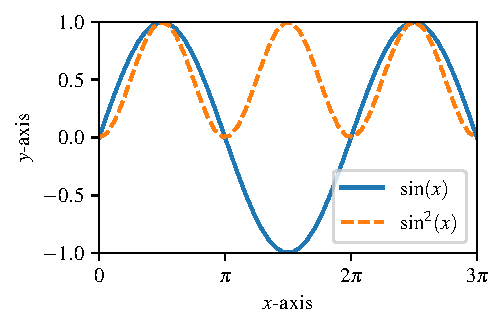
\includegraphics{myplot}
\caption{\label{fig:matplotlib} A plot created with PythonTeX and Matplotlib}
\end{figure}

\begin{pylabcode}
import os 
import pandas as pd
currentWorkingDir =  os.getcwd()
outputDataDir = currentWorkingDir + '/dep/kalman-soc/data/'
dfProcessedSensorDataEnhanced = pd.read_csv(outputDataDir + 'EVLKpN_20210817-20210830_enhanced_processed_sensor_data.zip')  

#Matplotlib
dfProcessedSensorDataEnhanced.plot()
plt.show()
savefig('matplotoverview.pdf', bbox_inches='tight')

#Plotly
pd.options.plotting.backend = "plotly"
fig = dfProcessedSensorDataEnhanced.plot()
fig.update_layout(title_text='<b> Overview  </b>', title_x=0.5)
fig.show()
fig.write_image("overview.pdf")
\end{pylabcode}
	
\begin{figure}[!ht]
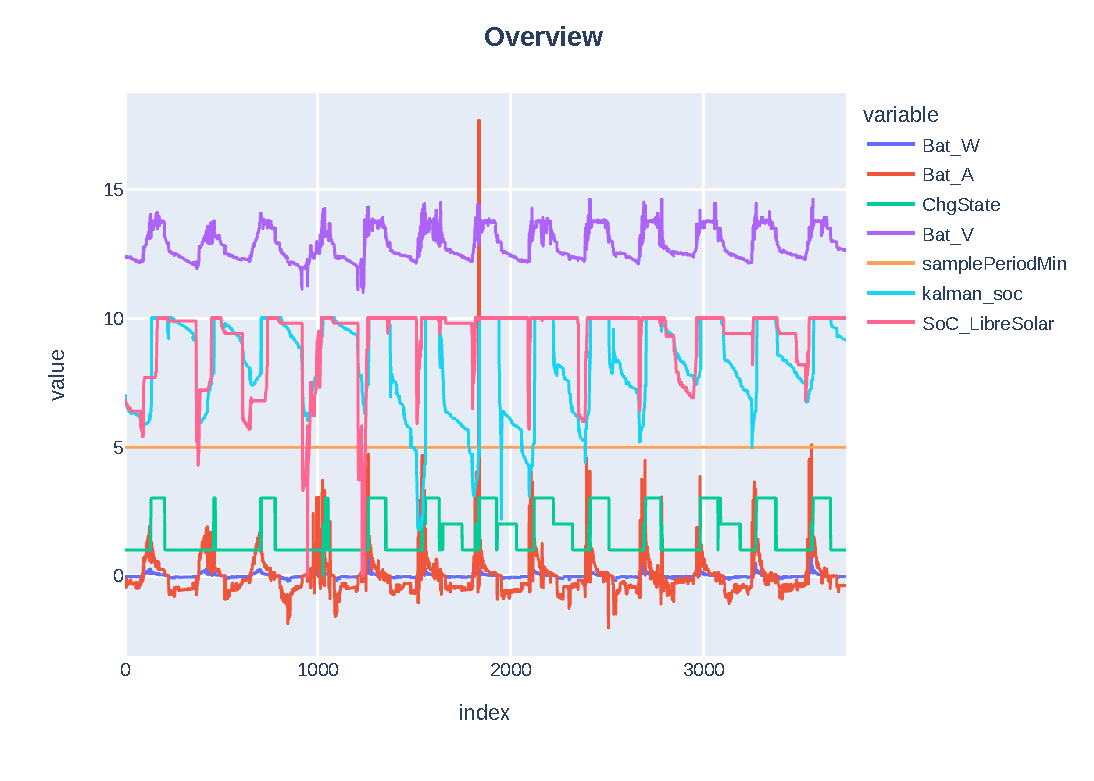
\includegraphics{overview}
\caption{\label{fig:overview} Overview of data}
\end{figure}

\begin{figure}[!ht]

\includegraphics{matplotoverview}
\caption{\label{fig:overview} Overview of data}
\end{figure}

\chapter{Outlook}

Promising articles and/or methods for online parameter estimation: \\ 

\textbf{online parameter estimation} from the ARX model {tran2017state}

\cite{wang2021augmented}
{xia2018online}
